\chapter{ Обзор литературы} \label{chapt1}
\section{ Графен}
Углерод является одним из самых распространенных веществ на Земле.  Он является частью огромного числа органических соединений, а также способен образовывать различные кристаллические структуры, такие как графит, алмаз, фуллерены и так далее. Такое разнообразие обусловлено особенностями электронной структуры углерода. В основном состоянии он находится в конфигурации $1s^22s^22p^2$.  При образовании ковалентной связи углерод переходит в возбужденное состояние $1s^22s^12p^3$. Повышение энергии при этом является оправданным, так как приводит к повышению энергии связи углерода с соседями.

	Для атома углерода возможны различные варианты гибридизации $s$  и $p$ орбиталей. Так, $sp^3$  гибридизация приводит к образованию алмаза, $sp^2$ гибридизация характерна для графита, а $sp$ гибридизация — для карбина.
	В случае смешения одной  $s$ и двух $p$ волновых функций образуются 3 гибридные  $sp^2$ орбитали, лежащие в одной плоскости. Они участвуют в образовании $\sigma$ связей. Оставшаяся $p_z$ орбиталь располагается перпендикулярно $sp^2$ плоскости и принимает участие в образовании  $\pi$ связи. Именно  $sp^2$ гибридизация ответственна за формирование графена. Графен — это двумерный материал, представляющий собой моноатомный слой углерода, обладающий сотовой структурой.
 \begin{figure}[ht] 
  \center
  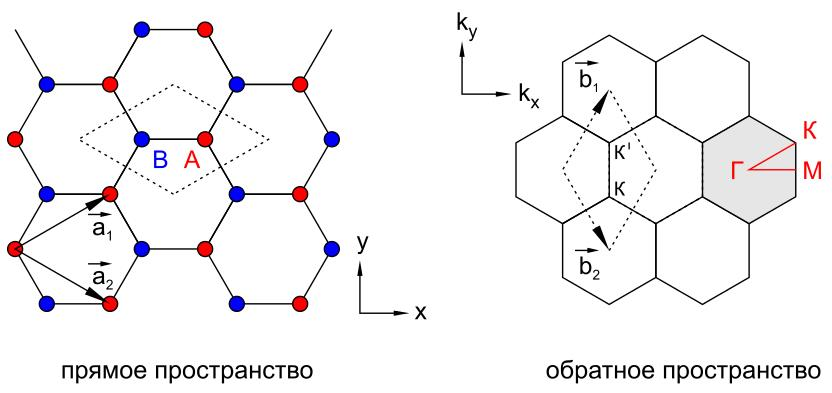
\includegraphics [scale=0.47] {11}
  \caption{Решётка графена в прямом и обратном пространстве.} 
  \label{img:11}  
\end{figure}

	Элементарная ячейка графена состоит из двух неэквивалентных атомов, образующих две подрешетки (Рис.\ref{img:11}). Используя вектора трансляции, невозможно получить одну подрешетку из другой. С другой стороны, атомы разных подрешеток имеют одинаковое окружение и являются в этом смысле эквивалентными. Постоянная решетки равна 2.46 Å, расстояние между двумя ближайшими атомами 1.42 Å. Обратная решетка также является сотовой структурой, форма первой зоны Бриллюэна — шестиугольник (Рис.\ref{img:11}).\cite{0953-8984-29-46-465901}
	
	Первые расчеты электронной структуры графена были проведены в 1947 году в приближении сильной связи \cite{1}. Четыре валентные орбитали каждого атома участвуют в образовании трех $\sigma$ и одной $\pi$ связи. При этом особый интерес представляет дисперсия $\pi$ состояний. Зонная структура графена представлена на Рис.\ref{img:12}.
 \begin{figure}[ht] 
  \center
  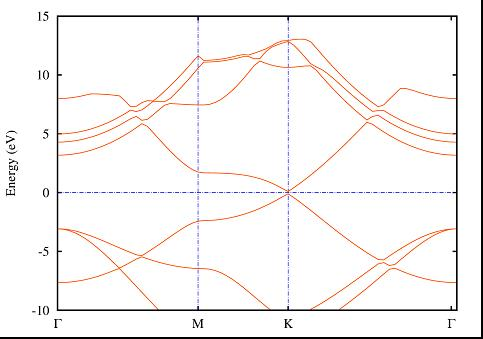
\includegraphics [scale=0.77] {12}
  \caption{Зонная структура графена, построенная вдоль высокосимметричных направлений первой зоны Бриллюэна.} 
  \label{img:12}  
\end{figure}

	Главной особенностью электронной структуры графена является наличие линейной дисперсии $\pi$-состояний вблизи точки К. Оба атома элементарной ячейки отдают по электрону для формирования  зон, вследствие чего связывающая $\pi$ орбиталь оказывается полностью заполненной, а разрыхляющая $\pi*$ орбиталь полностью пустой.  В точке К на уровне Ферми заполненный и незаполненный конус касаются друг друга. Наблюдается вырождение валентной зоны и зоны проводимости. Поэтому графен относят к бесщелевым полупроводникам. Коническая поверхность $E(k)$ вблизи точки К называется конусом Дирака. 
	
	Графен механически прочен, химически стоек и обладает рекордно высокой подвижностью носителей заряда. В силу выдающихся свойств он является чрезвычайно привлекательным для применений в электронике \cite{2}
\section{ Графен на подложке} \label{chapt_graphene-sic}
Линейный закон дисперсии вблизи точек касания валентной зоны и зоны проводимости присущ идеальному графену. В реальности графен всегда находится на подложке, с которой взаимодействует. Возникающие при этом модификации свойств графена являются следствием физико-химических свойств материала подложки. Для того чтобы научиться контролируемо модифицировать свойства графена, важно понимать, как именно происходит взаимодействие графена и вещества, на котором он находится. 

Для синтеза графена на металлических подложках широко используется метод химического осаждения из газовой фазы (CVD). Плотноупакованные грани Ni(111) и Co(0001) имеют постоянные решетки, близкие к постоянной решетки графена, что позволяет осуществлять рост высококачественного графена большой площади и делает эти интерфейсы удобными объектами исследования. Помимо этих двух металлов, графен может быть успешно синтезирован на Cu, Ir, Ru, Rh и Au. Дальнейшая модификация свойств графена может быть проведена с использованием процесса интеркаляции, который описан в следующем разделе.

	Наибольшее внимание уделялось системе графен/Ni(111) \cite{3,4,5,6,7,8,9,10}, что в значительной степени обусловлено возможностью формирования высококачественного графена на никеле методом химического осаждения из газовой фазы. В силу почти идеального соответствия постоянных решетки графена и никеля (отличие составляет менее 1,5 процентов) образуется плоская структура $p$(1 x 1) \cite{3}. 


	Экспериментальное и теоретическое исследование графена на никеле показало, что наличие подложки оказывает существенное влияние на его электронную структуру. По сравнению со структурой графита она сдвинута в сторону бÓльших энергий связи на 3 eV. Это обусловлено гибридизацией 3d состояний Ni с $p_z$ состояниями графена \cite{6}. Показано также, что вследствие сильного взаимодействия графена с металлической подложкой происходит значительная модификация электронной структуры графена и разрушение линейной дисперсионной зависимости $p_z$ состояний графена вблизи точки K зоны Бриллюэна. Перекрытие $\pi$ орбиталей углерода с $3d$ орбиталями никеля по энергии и в прямом и обратном пространстве приводит к тому, что в окрестности точки К зоны Бриллюэна появляется несколько гибридных состояний. Образующиеся гибридные орбитали обладают различной симметрией, и поэтому вырождение в точке К снимается через образование зазора. 
	
	
	Общий подход к пониманию электронной структуры графена на металлической подложке предложен в работе \cite{9}. В случае адсорбции графена на sp-металлах sp-электроны металла заполняют конус Дирака, что ведет к его смещению в область больших энергий связи и n-допированию графена.  Величина этого смещения, а также равновесное расстояние между графеном и подложкой зависит от разности работ выхода металла и графена. При этом линейная дисперсия $\pi$-состояний углерода остается ненарушенной. 
	
	Иная ситуация реализуется в случае взаимодействия графена с металлами с незаполненной 3d оболочкой. При перестройке электронной структуры графена происходят два процесса. Сначала, как и при взаимодействии с sp-металлами, конус Дирака смещается вследствие его заполнения sp-электронами подложки. В результате $\pi$-состояния углерода начинают перекрываться с 3d состояниями металла по шкале энергий. Вследствие этого происходит гибридизация этих состояний, и, следовательно, разрушение линейной дисперсии $\pi$-состояний вблизи точки К. 
\begin{figure}[ht] 
  \center
  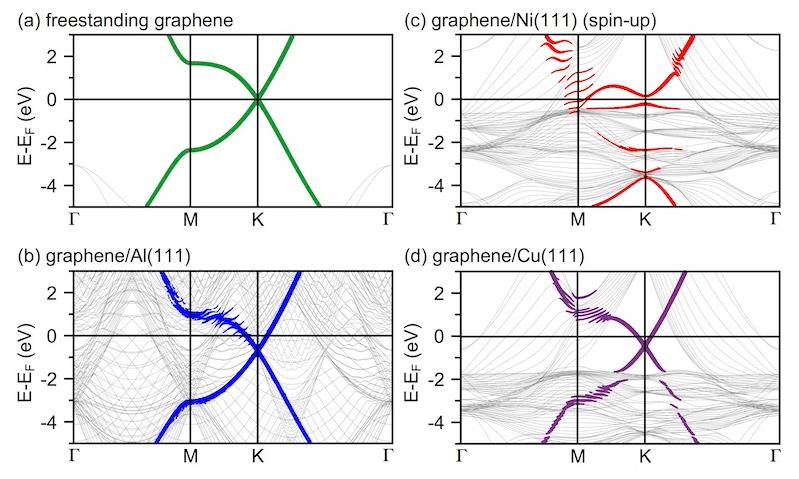
\includegraphics [scale=0.67] {25}
  \caption{Электронная структура свободного графена (a), электронная структура систем графен/Al(111) (b), графен/Ni(111) (с), графен/Сu(111) (d)  \cite{10}.} 
  \label{img:25}  
\end{figure}
	Выводы, сделанные для адсорбции графена на sp-металлах и металлах с незакрытой d-оболочкой, могут быть обобщены на случай взаимодействия графена с металлом с закрытой d-оболочкой.  Начальное допирование графена обусловлено sp-электронами металла. Заполненная d-оболочка оказывается расположена ниже точки Дирака, поэтому образование гибридных орбиталей в местах перекрытия $\pi$-состояний углерода и d-состояний металла не затрагивает конус Дирака.
	
	Приведенные рассуждения проиллюстрированы на Рис.\ref{img:25}. Зонная структура свободного графена показана на Рис. \ref{img:25} а. Энергетическая структура системы графен/Al(111), рассчитанная из первых принципов, приведена на Рис. \ref{img:25} b. Вклад $\pi$-состояний углерода выделен  синим цветом. Видно, что энергетическая структура $\pi$-состояний фактически повторяет дисперсионную характеристику свободнолежащего графена. Зонная структура системы графен/Ni(111) значительно видоизменена по сравнению с предыдущим случаем (Рис. \ref{img:25} c): из-за гибридизации линейная дисперсия $\pi$-состояний нарушается, и образуется несколько гибридных состояний. Наконец, энергетическая структура системы графен/Cu(111) показана на Рис. \ref{img:25} d. Видно, что в этом случае гибридизация не затрагивает конус Дирака в точке К. 
	
Другим популярным методом синтеза графена является термическое разложение карбида кремния. Данный способ позволяет получать высококачественный графен большой площади \cite{Davydov2017} на диэлектрической подложке. 
\begin{figure}[ht] 
  \center
  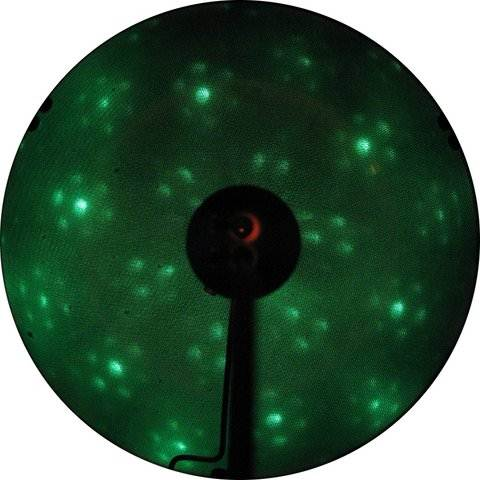
\includegraphics [scale=0.67] {gr-sic-leed}
  \caption{Картина дифракции медленных электронов для системы графен/SiC(0001)} 
  \label{img:leed_sic}  
\end{figure}
При этом между графеном и подложкой образуется буферный слой, представляющий собой графеноподобный слой атомов углерода, связанный с атомами кремния подложки. Расстояние между атомами буферного слоя и атомами кремния изменяется от 1.98Å до 2.25Å   А. В то же время расстояние между графеном и буферным слоем оказывается сравнимым с межплоскостным расстоянием в графите и составляет 3.15Å. В силу несоответствия постоянных решетки карбида кремния и графена возникает суперструктура $p(6\sqrt{3}\times6\sqrt{3})R30^{\circ}$, соответствующая наложению 169 ячеек графена на 108 ячеек подложки. Данная суперструктура проявляется как на картинах дифракции медленных электронов (Рис. \ref{img:leed_sic}), так и на на изображениях, снятых с помощью сканирующего туннельного микроскопа \cite{ab_initio_stm}.
\begin{figure}[ht] 
  \center
  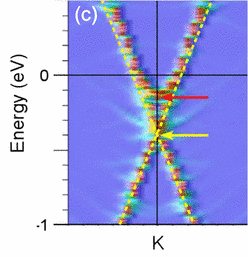
\includegraphics [scale=1] {gr-sic-dft}
  \caption{Фрагмент расчета зонной структуры системы графен/SiC(0001) из работы \cite{PhysRevLett.105.085502}.} 
  \label{img:gr-sic-dft}  
\end{figure}
Электронная структура графена в этом случае также оказывается изменена по сравнению со случаем свободного графена без подложки: конус Дирака смещается на 0.45 eV в сторону больших энергий связи, а состояния атомов углерода буферного слоя расположены на несколько электронвольт ниже уровня Ферми, что говорит о сильной связи этих атомов с атомами кремния \cite{AGRAWAL2013102}.
Наличие буферного слоя обуславливает основной недостаток графена, сформированного на карбиде кремния: рассеяние электронов на атомах буферного слоя ухудшает его транспортные свойства.




	
\section{ Интеркаляция графена} \label{chapt3}
Одним из перспективных способов целенаправленного изменения электронных и магнитных свойств интерфейса графен/подложка является интеркаляция его атомами или молекулами других веществ, т.е. внедрение инородных частиц под графен. Для активации процесса интеркаляции, как правило, необходим отжиг предварительно нанесенной на графен пленки инородного вещества. К настоящему времени имеется целый ряд работ, демонстрирующих большой потенциал данного способа модификации графена. Так, например, показано, что интеркаляция графена благородными металлами \cite{10,11} или атомами водорода \cite{12} может быть использована для уменьшения взаимодействия между графеном и подложкой, вплоть до восстановления электронных свойств свободного графена. В то же время интеркаляция  щелочными металлами является  эффективным средством управления уровнем электронного допирования графена \cite{13}. Наконец, интеркаляция графена атомами ферромагнитных металлов может приводить к появлению у него магнитных свойств \cite{8}. Этот способ также весьма перспективен для изготовления структур типа графен/ферромагнитный металл, обладающих перпендикулярной магнитной анизотропией \cite{14,15,16}. Ввиду того, что такие структуры представляют большой научный и практический интерес, графен, сформированный на поверхности магнитных металлов стал объектом активных исследований в последние годы.
\begin{figure}[ht] 
  \center
  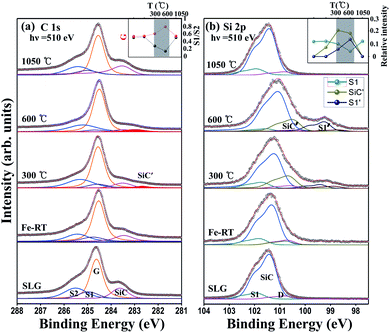
\includegraphics [scale=1] {c1s}
  \caption{Спектры С $1s$ и Si $2p$, полученные при различных температурах отжига в работе \cite{C3NR04178F}}. 
  \label{img:c1s}  
\end{figure}

	Влияние интеркаляции железа на атомное строение, электронную структуру и магнитные свойства интерфейса графен/Ni(111) исследовалось в работах \cite{17,18}.  Атомная структура и электронное строение интеркалированных слоев железа исследованы в работе \cite{19}, авторы которой использовали методы ДМЭ и рентгеновской ФЭС, а также провели теоретические расчеты, выполненные из первых принципов. Установлено, что пленки железа толщиной в один и два монослоя имеют такую же ГЦК структуру, как и подложка Ni(111), а атомы углерода располагаются над атомами железа в тех же местах, что и над атомами никелевой подложки. При этом, как и в случае чистого никеля, электронные состояния графена и железа сильно гибридизированы. Показано также, что внедрение под графен одного монослоя (ML) атомов железа резко меняет магнитный отклик графенового слоя и повышает магнитный момент атомов углерода \cite{20}. 
	Однако в силу особенностей взаимодействия графена с металлом линейный закон дисперсии в данной системе оказывается нарушен. Одним из способов восстановления электронной структуры графена является его дальнейшая интеркаляция атомами кремния. В работе \cite{PhysRevB.94.245421} показано, что внедрение $\frac{1}{3}$ML кремния способствует восстановлению графена в квазисвободное состояние.


\begin{figure}[ht] 
  \center
  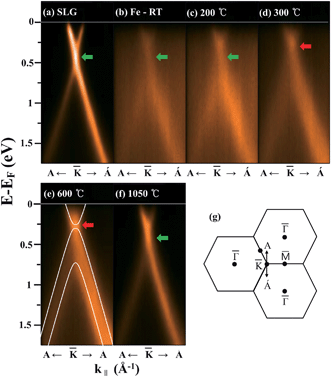
\includegraphics [scale=1] {arpes}
  \caption{Спектры фотоэлектронной спектроскопии с угловым разрешением, полученные при различных температурах отжига в работе \cite{C3NR04178F}}. 
  \label{img:arpes}  
\end{figure}

Альтернативным путем создания интерфейса графен/ферромагнетик является интеркаляция атомами металла графена, сформированного на карбиде кремния. Внедрение атомов железа в систему графен/SiC(0001) ранее исследовалось в работе \cite{C3NR04178F}, авторы которой установили, что при отжиге до температуры 600$^o$С атомы железа проникают под буферный слой, что подтверждается как экспериментальными данными, так и теоретическими расчетами. Так, из анализа фотоэлектронных спектров становится ясно, что при внедрении железа пропадают связи атомов буферного слоя с подложкой. Особый интерес представляет спектральная линия C $1s$, которая согласно данным работы \cite{PhysRevB.77.155303} включает в себя четыре компоненты. Наиболее интенсивная из них (мода G) соответствует графену. Вторая компонента (SiC) относится к атомам углерода в карбиде кремния. Наконец, моды S1 и S2 соответствуют двум типам атомов углерода в буферном слое, находящемся между графеном и верхним слоем атомов SiC(0001). При этом компонента S1 относится к тем атомам углерода, которые связаны висячими связями с нижележащим слоем SiC, а мода S2 соответствует атомам углерода, не связанным с этим слоем. После интеркаляции железа вклады всех мод, кроме G, значительно ослабляются (Рис. \ref{img:c1s}). 

Дополнительным свидетельством интеркаляции атомов железа под графен является отсутствие окисления полученного интерфейса после выдерживания в кислороде. Утверждается, что буферный слой отделяется от подложки, и на поверхности образуется двухслойный графен. Это должно приводить к возникновению характерных параболических дисперсионных кривых в окрестности точки К. Однако на спектрах фотоэлектронной спектроскопии с угловым разрешением видно, что после интеркаляции железа дисперсия $\pi$-состояний углерода лишь становится диффузной, размытой (Рис. \ref{img:arpes}).   



\section{ Выводы из обзора и постановка задач исследования} \label{chapt3}
Несмотря на растущий интерес исследователей к получению структур типа графен/ферромагнетик/диэлектрик, исследованию системы графен/Fe/SiC(0001) посвящена только работа \cite{C3NR04178F}. В ней показана возможность интеркалирования графена, выращенного на карбиде кремния, железом. При этом утверждается, что буферный слой при этом отрывается от подложки, и на поверхности интерфейса формируется квазисвободный двухслойный графен. Однако остается невыясненной локализация атомов железа в пленке. Кроме того, неясно, как интеркаляция атомов железа влияет на электронную структуру буферного слоя. В соответствии с литературными данными, в результате взаимодействия атомов буферного слоя и железа должны возникать гибридные орбитали, и, следовательно, буферный слой должен быть сильно связан с подложкой. Таким образом, ряд вопросов остается невыясненным. 

Целью настоящей диссертации стало получение новых знаний о системе графен/Fe/SiC(0001).

В соответствии с целью работы были поставлены следующие задачи:

1. изучение оптимальных условий формирования структуры графен/Fe/SiC(0001);

2. установление мест локализации атомов железа;

3. проведение первопринципных расчетов электронной структуры систем графен/SiC(0001) и графен/Fe/SiC(0001).

